\documentclass[11pt]{article}

    \usepackage[breakable]{tcolorbox}
    \usepackage{parskip} % Stop auto-indenting (to mimic markdown behaviour)
    
    \usepackage{iftex}
    \ifPDFTeX
    	\usepackage[T1]{fontenc}
    	\usepackage{mathpazo}
    \else
    	\usepackage{fontspec}
    \fi

    % Basic figure setup, for now with no caption control since it's done
    % automatically by Pandoc (which extracts ![](path) syntax from Markdown).
    \usepackage{graphicx}
    % Maintain compatibility with old templates. Remove in nbconvert 6.0
    \let\Oldincludegraphics\includegraphics
    % Ensure that by default, figures have no caption (until we provide a
    % proper Figure object with a Caption API and a way to capture that
    % in the conversion process - todo).
    \usepackage{caption}
    \DeclareCaptionFormat{nocaption}{}
    \captionsetup{format=nocaption,aboveskip=0pt,belowskip=0pt}

    \usepackage{float}
    \floatplacement{figure}{H} % forces figures to be placed at the correct location
    \usepackage{xcolor} % Allow colors to be defined
    \usepackage{enumerate} % Needed for markdown enumerations to work
    \usepackage{geometry} % Used to adjust the document margins
    \usepackage{amsmath} % Equations
    \usepackage{amssymb} % Equations
    \usepackage{textcomp} % defines textquotesingle
    % Hack from http://tex.stackexchange.com/a/47451/13684:
    \AtBeginDocument{%
        \def\PYZsq{\textquotesingle}% Upright quotes in Pygmentized code
    }
    \usepackage{upquote} % Upright quotes for verbatim code
    \usepackage{eurosym} % defines \euro
    \usepackage[mathletters]{ucs} % Extended unicode (utf-8) support
    \usepackage{fancyvrb} % verbatim replacement that allows latex
    \usepackage{grffile} % extends the file name processing of package graphics 
                         % to support a larger range
    \makeatletter % fix for old versions of grffile with XeLaTeX
    \@ifpackagelater{grffile}{2019/11/01}
    {
      % Do nothing on new versions
    }
    {
      \def\Gread@@xetex#1{%
        \IfFileExists{"\Gin@base".bb}%
        {\Gread@eps{\Gin@base.bb}}%
        {\Gread@@xetex@aux#1}%
      }
    }
    \makeatother
    \usepackage[Export]{adjustbox} % Used to constrain images to a maximum size
    \adjustboxset{max size={0.9\linewidth}{0.9\paperheight}}

    % The hyperref package gives us a pdf with properly built
    % internal navigation ('pdf bookmarks' for the table of contents,
    % internal cross-reference links, web links for URLs, etc.)
    \usepackage{hyperref}
    % The default LaTeX title has an obnoxious amount of whitespace. By default,
    % titling removes some of it. It also provides customization options.
    \usepackage{titling}
    \usepackage{longtable} % longtable support required by pandoc >1.10
    \usepackage{booktabs}  % table support for pandoc > 1.12.2
    \usepackage[inline]{enumitem} % IRkernel/repr support (it uses the enumerate* environment)
    \usepackage[normalem]{ulem} % ulem is needed to support strikethroughs (\sout)
                                % normalem makes italics be italics, not underlines
    \usepackage{mathrsfs}
    

    
    % Colors for the hyperref package
    \definecolor{urlcolor}{rgb}{0,.145,.698}
    \definecolor{linkcolor}{rgb}{.71,0.21,0.01}
    \definecolor{citecolor}{rgb}{.12,.54,.11}

    % ANSI colors
    \definecolor{ansi-black}{HTML}{3E424D}
    \definecolor{ansi-black-intense}{HTML}{282C36}
    \definecolor{ansi-red}{HTML}{E75C58}
    \definecolor{ansi-red-intense}{HTML}{B22B31}
    \definecolor{ansi-green}{HTML}{00A250}
    \definecolor{ansi-green-intense}{HTML}{007427}
    \definecolor{ansi-yellow}{HTML}{DDB62B}
    \definecolor{ansi-yellow-intense}{HTML}{B27D12}
    \definecolor{ansi-blue}{HTML}{208FFB}
    \definecolor{ansi-blue-intense}{HTML}{0065CA}
    \definecolor{ansi-magenta}{HTML}{D160C4}
    \definecolor{ansi-magenta-intense}{HTML}{A03196}
    \definecolor{ansi-cyan}{HTML}{60C6C8}
    \definecolor{ansi-cyan-intense}{HTML}{258F8F}
    \definecolor{ansi-white}{HTML}{C5C1B4}
    \definecolor{ansi-white-intense}{HTML}{A1A6B2}
    \definecolor{ansi-default-inverse-fg}{HTML}{FFFFFF}
    \definecolor{ansi-default-inverse-bg}{HTML}{000000}

    % common color for the border for error outputs.
    \definecolor{outerrorbackground}{HTML}{FFDFDF}

    % commands and environments needed by pandoc snippets
    % extracted from the output of `pandoc -s`
    \providecommand{\tightlist}{%
      \setlength{\itemsep}{0pt}\setlength{\parskip}{0pt}}
    \DefineVerbatimEnvironment{Highlighting}{Verbatim}{commandchars=\\\{\}}
    % Add ',fontsize=\small' for more characters per line
    \newenvironment{Shaded}{}{}
    \newcommand{\KeywordTok}[1]{\textcolor[rgb]{0.00,0.44,0.13}{\textbf{{#1}}}}
    \newcommand{\DataTypeTok}[1]{\textcolor[rgb]{0.56,0.13,0.00}{{#1}}}
    \newcommand{\DecValTok}[1]{\textcolor[rgb]{0.25,0.63,0.44}{{#1}}}
    \newcommand{\BaseNTok}[1]{\textcolor[rgb]{0.25,0.63,0.44}{{#1}}}
    \newcommand{\FloatTok}[1]{\textcolor[rgb]{0.25,0.63,0.44}{{#1}}}
    \newcommand{\CharTok}[1]{\textcolor[rgb]{0.25,0.44,0.63}{{#1}}}
    \newcommand{\StringTok}[1]{\textcolor[rgb]{0.25,0.44,0.63}{{#1}}}
    \newcommand{\CommentTok}[1]{\textcolor[rgb]{0.38,0.63,0.69}{\textit{{#1}}}}
    \newcommand{\OtherTok}[1]{\textcolor[rgb]{0.00,0.44,0.13}{{#1}}}
    \newcommand{\AlertTok}[1]{\textcolor[rgb]{1.00,0.00,0.00}{\textbf{{#1}}}}
    \newcommand{\FunctionTok}[1]{\textcolor[rgb]{0.02,0.16,0.49}{{#1}}}
    \newcommand{\RegionMarkerTok}[1]{{#1}}
    \newcommand{\ErrorTok}[1]{\textcolor[rgb]{1.00,0.00,0.00}{\textbf{{#1}}}}
    \newcommand{\NormalTok}[1]{{#1}}
    
    % Additional commands for more recent versions of Pandoc
    \newcommand{\ConstantTok}[1]{\textcolor[rgb]{0.53,0.00,0.00}{{#1}}}
    \newcommand{\SpecialCharTok}[1]{\textcolor[rgb]{0.25,0.44,0.63}{{#1}}}
    \newcommand{\VerbatimStringTok}[1]{\textcolor[rgb]{0.25,0.44,0.63}{{#1}}}
    \newcommand{\SpecialStringTok}[1]{\textcolor[rgb]{0.73,0.40,0.53}{{#1}}}
    \newcommand{\ImportTok}[1]{{#1}}
    \newcommand{\DocumentationTok}[1]{\textcolor[rgb]{0.73,0.13,0.13}{\textit{{#1}}}}
    \newcommand{\AnnotationTok}[1]{\textcolor[rgb]{0.38,0.63,0.69}{\textbf{\textit{{#1}}}}}
    \newcommand{\CommentVarTok}[1]{\textcolor[rgb]{0.38,0.63,0.69}{\textbf{\textit{{#1}}}}}
    \newcommand{\VariableTok}[1]{\textcolor[rgb]{0.10,0.09,0.49}{{#1}}}
    \newcommand{\ControlFlowTok}[1]{\textcolor[rgb]{0.00,0.44,0.13}{\textbf{{#1}}}}
    \newcommand{\OperatorTok}[1]{\textcolor[rgb]{0.40,0.40,0.40}{{#1}}}
    \newcommand{\BuiltInTok}[1]{{#1}}
    \newcommand{\ExtensionTok}[1]{{#1}}
    \newcommand{\PreprocessorTok}[1]{\textcolor[rgb]{0.74,0.48,0.00}{{#1}}}
    \newcommand{\AttributeTok}[1]{\textcolor[rgb]{0.49,0.56,0.16}{{#1}}}
    \newcommand{\InformationTok}[1]{\textcolor[rgb]{0.38,0.63,0.69}{\textbf{\textit{{#1}}}}}
    \newcommand{\WarningTok}[1]{\textcolor[rgb]{0.38,0.63,0.69}{\textbf{\textit{{#1}}}}}
    
    
    % Define a nice break command that doesn't care if a line doesn't already
    % exist.
    \def\br{\hspace*{\fill} \\* }
    % Math Jax compatibility definitions
    \def\gt{>}
    \def\lt{<}
    \let\Oldtex\TeX
    \let\Oldlatex\LaTeX
    \renewcommand{\TeX}{\textrm{\Oldtex}}
    \renewcommand{\LaTeX}{\textrm{\Oldlatex}}
    % Document parameters
    % Document title
    \title{Pandas SQL-like functionality}
    
    
    
    
    
% Pygments definitions
\makeatletter
\def\PY@reset{\let\PY@it=\relax \let\PY@bf=\relax%
    \let\PY@ul=\relax \let\PY@tc=\relax%
    \let\PY@bc=\relax \let\PY@ff=\relax}
\def\PY@tok#1{\csname PY@tok@#1\endcsname}
\def\PY@toks#1+{\ifx\relax#1\empty\else%
    \PY@tok{#1}\expandafter\PY@toks\fi}
\def\PY@do#1{\PY@bc{\PY@tc{\PY@ul{%
    \PY@it{\PY@bf{\PY@ff{#1}}}}}}}
\def\PY#1#2{\PY@reset\PY@toks#1+\relax+\PY@do{#2}}

\expandafter\def\csname PY@tok@w\endcsname{\def\PY@tc##1{\textcolor[rgb]{0.73,0.73,0.73}{##1}}}
\expandafter\def\csname PY@tok@c\endcsname{\let\PY@it=\textit\def\PY@tc##1{\textcolor[rgb]{0.25,0.50,0.50}{##1}}}
\expandafter\def\csname PY@tok@cp\endcsname{\def\PY@tc##1{\textcolor[rgb]{0.74,0.48,0.00}{##1}}}
\expandafter\def\csname PY@tok@k\endcsname{\let\PY@bf=\textbf\def\PY@tc##1{\textcolor[rgb]{0.00,0.50,0.00}{##1}}}
\expandafter\def\csname PY@tok@kp\endcsname{\def\PY@tc##1{\textcolor[rgb]{0.00,0.50,0.00}{##1}}}
\expandafter\def\csname PY@tok@kt\endcsname{\def\PY@tc##1{\textcolor[rgb]{0.69,0.00,0.25}{##1}}}
\expandafter\def\csname PY@tok@o\endcsname{\def\PY@tc##1{\textcolor[rgb]{0.40,0.40,0.40}{##1}}}
\expandafter\def\csname PY@tok@ow\endcsname{\let\PY@bf=\textbf\def\PY@tc##1{\textcolor[rgb]{0.67,0.13,1.00}{##1}}}
\expandafter\def\csname PY@tok@nb\endcsname{\def\PY@tc##1{\textcolor[rgb]{0.00,0.50,0.00}{##1}}}
\expandafter\def\csname PY@tok@nf\endcsname{\def\PY@tc##1{\textcolor[rgb]{0.00,0.00,1.00}{##1}}}
\expandafter\def\csname PY@tok@nc\endcsname{\let\PY@bf=\textbf\def\PY@tc##1{\textcolor[rgb]{0.00,0.00,1.00}{##1}}}
\expandafter\def\csname PY@tok@nn\endcsname{\let\PY@bf=\textbf\def\PY@tc##1{\textcolor[rgb]{0.00,0.00,1.00}{##1}}}
\expandafter\def\csname PY@tok@ne\endcsname{\let\PY@bf=\textbf\def\PY@tc##1{\textcolor[rgb]{0.82,0.25,0.23}{##1}}}
\expandafter\def\csname PY@tok@nv\endcsname{\def\PY@tc##1{\textcolor[rgb]{0.10,0.09,0.49}{##1}}}
\expandafter\def\csname PY@tok@no\endcsname{\def\PY@tc##1{\textcolor[rgb]{0.53,0.00,0.00}{##1}}}
\expandafter\def\csname PY@tok@nl\endcsname{\def\PY@tc##1{\textcolor[rgb]{0.63,0.63,0.00}{##1}}}
\expandafter\def\csname PY@tok@ni\endcsname{\let\PY@bf=\textbf\def\PY@tc##1{\textcolor[rgb]{0.60,0.60,0.60}{##1}}}
\expandafter\def\csname PY@tok@na\endcsname{\def\PY@tc##1{\textcolor[rgb]{0.49,0.56,0.16}{##1}}}
\expandafter\def\csname PY@tok@nt\endcsname{\let\PY@bf=\textbf\def\PY@tc##1{\textcolor[rgb]{0.00,0.50,0.00}{##1}}}
\expandafter\def\csname PY@tok@nd\endcsname{\def\PY@tc##1{\textcolor[rgb]{0.67,0.13,1.00}{##1}}}
\expandafter\def\csname PY@tok@s\endcsname{\def\PY@tc##1{\textcolor[rgb]{0.73,0.13,0.13}{##1}}}
\expandafter\def\csname PY@tok@sd\endcsname{\let\PY@it=\textit\def\PY@tc##1{\textcolor[rgb]{0.73,0.13,0.13}{##1}}}
\expandafter\def\csname PY@tok@si\endcsname{\let\PY@bf=\textbf\def\PY@tc##1{\textcolor[rgb]{0.73,0.40,0.53}{##1}}}
\expandafter\def\csname PY@tok@se\endcsname{\let\PY@bf=\textbf\def\PY@tc##1{\textcolor[rgb]{0.73,0.40,0.13}{##1}}}
\expandafter\def\csname PY@tok@sr\endcsname{\def\PY@tc##1{\textcolor[rgb]{0.73,0.40,0.53}{##1}}}
\expandafter\def\csname PY@tok@ss\endcsname{\def\PY@tc##1{\textcolor[rgb]{0.10,0.09,0.49}{##1}}}
\expandafter\def\csname PY@tok@sx\endcsname{\def\PY@tc##1{\textcolor[rgb]{0.00,0.50,0.00}{##1}}}
\expandafter\def\csname PY@tok@m\endcsname{\def\PY@tc##1{\textcolor[rgb]{0.40,0.40,0.40}{##1}}}
\expandafter\def\csname PY@tok@gh\endcsname{\let\PY@bf=\textbf\def\PY@tc##1{\textcolor[rgb]{0.00,0.00,0.50}{##1}}}
\expandafter\def\csname PY@tok@gu\endcsname{\let\PY@bf=\textbf\def\PY@tc##1{\textcolor[rgb]{0.50,0.00,0.50}{##1}}}
\expandafter\def\csname PY@tok@gd\endcsname{\def\PY@tc##1{\textcolor[rgb]{0.63,0.00,0.00}{##1}}}
\expandafter\def\csname PY@tok@gi\endcsname{\def\PY@tc##1{\textcolor[rgb]{0.00,0.63,0.00}{##1}}}
\expandafter\def\csname PY@tok@gr\endcsname{\def\PY@tc##1{\textcolor[rgb]{1.00,0.00,0.00}{##1}}}
\expandafter\def\csname PY@tok@ge\endcsname{\let\PY@it=\textit}
\expandafter\def\csname PY@tok@gs\endcsname{\let\PY@bf=\textbf}
\expandafter\def\csname PY@tok@gp\endcsname{\let\PY@bf=\textbf\def\PY@tc##1{\textcolor[rgb]{0.00,0.00,0.50}{##1}}}
\expandafter\def\csname PY@tok@go\endcsname{\def\PY@tc##1{\textcolor[rgb]{0.53,0.53,0.53}{##1}}}
\expandafter\def\csname PY@tok@gt\endcsname{\def\PY@tc##1{\textcolor[rgb]{0.00,0.27,0.87}{##1}}}
\expandafter\def\csname PY@tok@err\endcsname{\def\PY@bc##1{\setlength{\fboxsep}{0pt}\fcolorbox[rgb]{1.00,0.00,0.00}{1,1,1}{\strut ##1}}}
\expandafter\def\csname PY@tok@kc\endcsname{\let\PY@bf=\textbf\def\PY@tc##1{\textcolor[rgb]{0.00,0.50,0.00}{##1}}}
\expandafter\def\csname PY@tok@kd\endcsname{\let\PY@bf=\textbf\def\PY@tc##1{\textcolor[rgb]{0.00,0.50,0.00}{##1}}}
\expandafter\def\csname PY@tok@kn\endcsname{\let\PY@bf=\textbf\def\PY@tc##1{\textcolor[rgb]{0.00,0.50,0.00}{##1}}}
\expandafter\def\csname PY@tok@kr\endcsname{\let\PY@bf=\textbf\def\PY@tc##1{\textcolor[rgb]{0.00,0.50,0.00}{##1}}}
\expandafter\def\csname PY@tok@bp\endcsname{\def\PY@tc##1{\textcolor[rgb]{0.00,0.50,0.00}{##1}}}
\expandafter\def\csname PY@tok@fm\endcsname{\def\PY@tc##1{\textcolor[rgb]{0.00,0.00,1.00}{##1}}}
\expandafter\def\csname PY@tok@vc\endcsname{\def\PY@tc##1{\textcolor[rgb]{0.10,0.09,0.49}{##1}}}
\expandafter\def\csname PY@tok@vg\endcsname{\def\PY@tc##1{\textcolor[rgb]{0.10,0.09,0.49}{##1}}}
\expandafter\def\csname PY@tok@vi\endcsname{\def\PY@tc##1{\textcolor[rgb]{0.10,0.09,0.49}{##1}}}
\expandafter\def\csname PY@tok@vm\endcsname{\def\PY@tc##1{\textcolor[rgb]{0.10,0.09,0.49}{##1}}}
\expandafter\def\csname PY@tok@sa\endcsname{\def\PY@tc##1{\textcolor[rgb]{0.73,0.13,0.13}{##1}}}
\expandafter\def\csname PY@tok@sb\endcsname{\def\PY@tc##1{\textcolor[rgb]{0.73,0.13,0.13}{##1}}}
\expandafter\def\csname PY@tok@sc\endcsname{\def\PY@tc##1{\textcolor[rgb]{0.73,0.13,0.13}{##1}}}
\expandafter\def\csname PY@tok@dl\endcsname{\def\PY@tc##1{\textcolor[rgb]{0.73,0.13,0.13}{##1}}}
\expandafter\def\csname PY@tok@s2\endcsname{\def\PY@tc##1{\textcolor[rgb]{0.73,0.13,0.13}{##1}}}
\expandafter\def\csname PY@tok@sh\endcsname{\def\PY@tc##1{\textcolor[rgb]{0.73,0.13,0.13}{##1}}}
\expandafter\def\csname PY@tok@s1\endcsname{\def\PY@tc##1{\textcolor[rgb]{0.73,0.13,0.13}{##1}}}
\expandafter\def\csname PY@tok@mb\endcsname{\def\PY@tc##1{\textcolor[rgb]{0.40,0.40,0.40}{##1}}}
\expandafter\def\csname PY@tok@mf\endcsname{\def\PY@tc##1{\textcolor[rgb]{0.40,0.40,0.40}{##1}}}
\expandafter\def\csname PY@tok@mh\endcsname{\def\PY@tc##1{\textcolor[rgb]{0.40,0.40,0.40}{##1}}}
\expandafter\def\csname PY@tok@mi\endcsname{\def\PY@tc##1{\textcolor[rgb]{0.40,0.40,0.40}{##1}}}
\expandafter\def\csname PY@tok@il\endcsname{\def\PY@tc##1{\textcolor[rgb]{0.40,0.40,0.40}{##1}}}
\expandafter\def\csname PY@tok@mo\endcsname{\def\PY@tc##1{\textcolor[rgb]{0.40,0.40,0.40}{##1}}}
\expandafter\def\csname PY@tok@ch\endcsname{\let\PY@it=\textit\def\PY@tc##1{\textcolor[rgb]{0.25,0.50,0.50}{##1}}}
\expandafter\def\csname PY@tok@cm\endcsname{\let\PY@it=\textit\def\PY@tc##1{\textcolor[rgb]{0.25,0.50,0.50}{##1}}}
\expandafter\def\csname PY@tok@cpf\endcsname{\let\PY@it=\textit\def\PY@tc##1{\textcolor[rgb]{0.25,0.50,0.50}{##1}}}
\expandafter\def\csname PY@tok@c1\endcsname{\let\PY@it=\textit\def\PY@tc##1{\textcolor[rgb]{0.25,0.50,0.50}{##1}}}
\expandafter\def\csname PY@tok@cs\endcsname{\let\PY@it=\textit\def\PY@tc##1{\textcolor[rgb]{0.25,0.50,0.50}{##1}}}

\def\PYZbs{\char`\\}
\def\PYZus{\char`\_}
\def\PYZob{\char`\{}
\def\PYZcb{\char`\}}
\def\PYZca{\char`\^}
\def\PYZam{\char`\&}
\def\PYZlt{\char`\<}
\def\PYZgt{\char`\>}
\def\PYZsh{\char`\#}
\def\PYZpc{\char`\%}
\def\PYZdl{\char`\$}
\def\PYZhy{\char`\-}
\def\PYZsq{\char`\'}
\def\PYZdq{\char`\"}
\def\PYZti{\char`\~}
% for compatibility with earlier versions
\def\PYZat{@}
\def\PYZlb{[}
\def\PYZrb{]}
\makeatother


    % For linebreaks inside Verbatim environment from package fancyvrb. 
    \makeatletter
        \newbox\Wrappedcontinuationbox 
        \newbox\Wrappedvisiblespacebox 
        \newcommand*\Wrappedvisiblespace {\textcolor{red}{\textvisiblespace}} 
        \newcommand*\Wrappedcontinuationsymbol {\textcolor{red}{\llap{\tiny$\m@th\hookrightarrow$}}} 
        \newcommand*\Wrappedcontinuationindent {3ex } 
        \newcommand*\Wrappedafterbreak {\kern\Wrappedcontinuationindent\copy\Wrappedcontinuationbox} 
        % Take advantage of the already applied Pygments mark-up to insert 
        % potential linebreaks for TeX processing. 
        %        {, <, #, %, $, ' and ": go to next line. 
        %        _, }, ^, &, >, - and ~: stay at end of broken line. 
        % Use of \textquotesingle for straight quote. 
        \newcommand*\Wrappedbreaksatspecials {% 
            \def\PYGZus{\discretionary{\char`\_}{\Wrappedafterbreak}{\char`\_}}% 
            \def\PYGZob{\discretionary{}{\Wrappedafterbreak\char`\{}{\char`\{}}% 
            \def\PYGZcb{\discretionary{\char`\}}{\Wrappedafterbreak}{\char`\}}}% 
            \def\PYGZca{\discretionary{\char`\^}{\Wrappedafterbreak}{\char`\^}}% 
            \def\PYGZam{\discretionary{\char`\&}{\Wrappedafterbreak}{\char`\&}}% 
            \def\PYGZlt{\discretionary{}{\Wrappedafterbreak\char`\<}{\char`\<}}% 
            \def\PYGZgt{\discretionary{\char`\>}{\Wrappedafterbreak}{\char`\>}}% 
            \def\PYGZsh{\discretionary{}{\Wrappedafterbreak\char`\#}{\char`\#}}% 
            \def\PYGZpc{\discretionary{}{\Wrappedafterbreak\char`\%}{\char`\%}}% 
            \def\PYGZdl{\discretionary{}{\Wrappedafterbreak\char`\$}{\char`\$}}% 
            \def\PYGZhy{\discretionary{\char`\-}{\Wrappedafterbreak}{\char`\-}}% 
            \def\PYGZsq{\discretionary{}{\Wrappedafterbreak\textquotesingle}{\textquotesingle}}% 
            \def\PYGZdq{\discretionary{}{\Wrappedafterbreak\char`\"}{\char`\"}}% 
            \def\PYGZti{\discretionary{\char`\~}{\Wrappedafterbreak}{\char`\~}}% 
        } 
        % Some characters . , ; ? ! / are not pygmentized. 
        % This macro makes them "active" and they will insert potential linebreaks 
        \newcommand*\Wrappedbreaksatpunct {% 
            \lccode`\~`\.\lowercase{\def~}{\discretionary{\hbox{\char`\.}}{\Wrappedafterbreak}{\hbox{\char`\.}}}% 
            \lccode`\~`\,\lowercase{\def~}{\discretionary{\hbox{\char`\,}}{\Wrappedafterbreak}{\hbox{\char`\,}}}% 
            \lccode`\~`\;\lowercase{\def~}{\discretionary{\hbox{\char`\;}}{\Wrappedafterbreak}{\hbox{\char`\;}}}% 
            \lccode`\~`\:\lowercase{\def~}{\discretionary{\hbox{\char`\:}}{\Wrappedafterbreak}{\hbox{\char`\:}}}% 
            \lccode`\~`\?\lowercase{\def~}{\discretionary{\hbox{\char`\?}}{\Wrappedafterbreak}{\hbox{\char`\?}}}% 
            \lccode`\~`\!\lowercase{\def~}{\discretionary{\hbox{\char`\!}}{\Wrappedafterbreak}{\hbox{\char`\!}}}% 
            \lccode`\~`\/\lowercase{\def~}{\discretionary{\hbox{\char`\/}}{\Wrappedafterbreak}{\hbox{\char`\/}}}% 
            \catcode`\.\active
            \catcode`\,\active 
            \catcode`\;\active
            \catcode`\:\active
            \catcode`\?\active
            \catcode`\!\active
            \catcode`\/\active 
            \lccode`\~`\~ 	
        }
    \makeatother

    \let\OriginalVerbatim=\Verbatim
    \makeatletter
    \renewcommand{\Verbatim}[1][1]{%
        %\parskip\z@skip
        \sbox\Wrappedcontinuationbox {\Wrappedcontinuationsymbol}%
        \sbox\Wrappedvisiblespacebox {\FV@SetupFont\Wrappedvisiblespace}%
        \def\FancyVerbFormatLine ##1{\hsize\linewidth
            \vtop{\raggedright\hyphenpenalty\z@\exhyphenpenalty\z@
                \doublehyphendemerits\z@\finalhyphendemerits\z@
                \strut ##1\strut}%
        }%
        % If the linebreak is at a space, the latter will be displayed as visible
        % space at end of first line, and a continuation symbol starts next line.
        % Stretch/shrink are however usually zero for typewriter font.
        \def\FV@Space {%
            \nobreak\hskip\z@ plus\fontdimen3\font minus\fontdimen4\font
            \discretionary{\copy\Wrappedvisiblespacebox}{\Wrappedafterbreak}
            {\kern\fontdimen2\font}%
        }%
        
        % Allow breaks at special characters using \PYG... macros.
        \Wrappedbreaksatspecials
        % Breaks at punctuation characters . , ; ? ! and / need catcode=\active 	
        \OriginalVerbatim[#1,codes*=\Wrappedbreaksatpunct]%
    }
    \makeatother

    % Exact colors from NB
    \definecolor{incolor}{HTML}{303F9F}
    \definecolor{outcolor}{HTML}{D84315}
    \definecolor{cellborder}{HTML}{CFCFCF}
    \definecolor{cellbackground}{HTML}{F7F7F7}
    
    % prompt
    \makeatletter
    \newcommand{\boxspacing}{\kern\kvtcb@left@rule\kern\kvtcb@boxsep}
    \makeatother
    \newcommand{\prompt}[4]{
        {\ttfamily\llap{{\color{#2}[#3]:\hspace{3pt}#4}}\vspace{-\baselineskip}}
    }
    

    
    % Prevent overflowing lines due to hard-to-break entities
    \sloppy 
    % Setup hyperref package
    \hypersetup{
      breaklinks=true,  % so long urls are correctly broken across lines
      colorlinks=true,
      urlcolor=urlcolor,
      linkcolor=linkcolor,
      citecolor=citecolor,
      }
    % Slightly bigger margins than the latex defaults
    
    \geometry{verbose,tmargin=1in,bmargin=1in,lmargin=1in,rmargin=1in}
    
    

\begin{document}
    
    \maketitle
    
    

    
    How to use Pandas for SQL-like actions

Part 1 - Overall review

Hessam Mohammad Hosseini

In this cheetsheet, I try to make readable and easy to use reference for
\href{https://en.wikipedia.org/wiki/SQL}{SQL} users aiming to explain
how to do similar action in \href{https://pandas.pydata.org/}{Pandas}.
My assumption is you know how to have your data as dataframe in Pandas.
As soon as you have a dataframe, you can quey like table in SQL.

Many possibilities are avaiable
\href{https://pandas.pydata.org/pandas-docs/stable/user_guide/io.html}{IO
Tools (CSV, EXCEL,DB connection \ldots)} but most important ones are
reading from Excel and CSV. For example, following will read file
address of which is \texttt{file\_address}, skip first row, consider
\texttt{Time} column to be parsed as \texttt{datetime} format and
consider \texttt{,} as thousands identifer while reading file.
\texttt{df\ =\ \ pd.read\_csv(file\_name,skiprows=1,parse\_dates={[}\textquotesingle{}Time\textquotesingle{}{]},thousands=\textquotesingle{},\textquotesingle{})}

\begin{enumerate}
\def\labelenumi{\arabic{enumi}.}
\item
  \href{https://pandas.pydata.org/pandas-docs/stable/reference/api/pandas.read_csv.html}{Read
  csv} Functions has lots of useful options to fasilitate work. Here are
  options for \texttt{read\_csv}. Many of :
  \texttt{df\ =\ pandas.read\_csv(filepath\_or\_buffer,\ sep=\textquotesingle{},\ \textquotesingle{},\ delimiter=None,\ header=\textquotesingle{}infer\textquotesingle{},\ names=None,\ index\_col=None,\ usecols=None,\ squeeze=False,\ prefix=None,\ mangle\_dupe\_cols=True,\ dtype=None,\ engine=None,\ converters=None,\ true\_values=None,\ false\_values=None,\ skipinitialspace=False,\ skiprows=None,\ skipfooter=0,\ nrows=None,\ na\_values=None,\ keep\_default\_na=True,\ na\_filter=True,\ verbose=False,\ skip\_blank\_lines=True,\ parse\_dates=False,\ infer\_datetime\_format=False,\ keep\_date\_col=False,\ date\_parser=None,\ dayfirst=False,\ iterator=False,\ chunksize=None,\ compression=\textquotesingle{}infer\textquotesingle{},\ thousands=None,\ decimal=b\textquotesingle{}.\textquotesingle{},\ lineterminator=None,\ quotechar=\textquotesingle{}"\textquotesingle{},\ quoting=0,\ doublequote=True,\ escapechar=None,\ comment=None,\ encoding=None,\ dialect=None,\ tupleize\_cols=None,\ error\_bad\_lines=True,\ warn\_bad\_lines=True,\ delim\_whitespace=False,\ low\_memory=True,\ memory\_map=False,\ float\_precision=None)}
\item
  \href{https://pandas.pydata.org/pandas-docs/stable/reference/api/pandas.read_excel.html\#pandas.read_excel}{Read
  excel} Functions has lots of useful options to fasilitate work. Here
  are options for \texttt{read\_excel}:
  \texttt{df\ =\ pandas.read\_excel(io,\ sheet\_name=0,\ header=0,\ names=None,\ index\_col=None,\ parse\_cols=None,\ usecols=None,\ squeeze=False,\ dtype=None,\ engine=None,\ converters=None,\ true\_values=None,\ false\_values=None,\ skiprows=None,\ nrows=None,\ na\_values=None,\ keep\_default\_na=True,\ verbose=False,\ parse\_dates=False,\ date\_parser=None,\ thousands=None,\ comment=None,\ skip\_footer=0,\ skipfooter=0,\ convert\_float=True,\ mangle\_dupe\_cols=True,\ **kwds)}
\end{enumerate}

I tried to summerized and add to what was available on
\href{https://pandas.pydata.org/pandas-docs/stable/getting_started/comparison/comparison_with_sql.html}{Pandas
comparison with SQL} aiming to simplify understanding. For details on
functionality, please check and review
\href{http://pandas.pydata.org/pandas-docs/stable}{Pandas
documentation}.

    \hypertarget{select}{%
\subsection{1. SELECT}\label{select}}

    \begin{longtable}[]{@{}ccc@{}}
\toprule
\begin{minipage}[b]{0.29\columnwidth}\centering
SQL Sample\strut
\end{minipage} & \begin{minipage}[b]{0.34\columnwidth}\centering
Pandas Sample\strut
\end{minipage} & \begin{minipage}[b]{0.29\columnwidth}\centering
\strut
\end{minipage}\tabularnewline
\midrule
\endhead
\begin{minipage}[t]{0.29\columnwidth}\centering
\texttt{select\ *}\texttt{from\ table}\strut
\end{minipage} & \begin{minipage}[t]{0.34\columnwidth}\centering
\texttt{table}\strut
\end{minipage} & \begin{minipage}[t]{0.29\columnwidth}\centering
\strut
\end{minipage}\tabularnewline
\begin{minipage}[t]{0.29\columnwidth}\centering
\texttt{select\ distinct\ c5}\texttt{from\ table}\strut
\end{minipage} & \begin{minipage}[t]{0.34\columnwidth}\centering
\texttt{table{[}\textquotesingle{}c5\textquotesingle{}{]}.unique()} or
\texttt{table{[}{[}\textquotesingle{}c5\textquotesingle{}{]}{]}.drop\_duplicates()}\strut
\end{minipage} & \begin{minipage}[t]{0.29\columnwidth}\centering
\strut
\end{minipage}\tabularnewline
\begin{minipage}[t]{0.29\columnwidth}\centering
\texttt{select\ c1,\ c2,c10}\texttt{from\ table}\strut
\end{minipage} & \begin{minipage}[t]{0.34\columnwidth}\centering
\texttt{df{[}{[}c1,\ c2,c10{]}{]}}\strut
\end{minipage} & \begin{minipage}[t]{0.29\columnwidth}\centering
\strut
\end{minipage}\tabularnewline
\begin{minipage}[t]{0.29\columnwidth}\centering
\texttt{select\ c10,\ c2,\ c1}\texttt{from\ table}\strut
\end{minipage} & \begin{minipage}[t]{0.34\columnwidth}\centering
\texttt{df{[}{[}c10,\ c1,\ c2{]}{]}}\strut
\end{minipage} & \begin{minipage}[t]{0.29\columnwidth}\centering
\strut
\end{minipage}\tabularnewline
\begin{minipage}[t]{0.29\columnwidth}\centering
\texttt{select\ c10,\ c2*12\ -\ c1\ +\ c6}\texttt{from\ table}\strut
\end{minipage} & \begin{minipage}[t]{0.34\columnwidth}\centering
\texttt{df{[}\textquotesingle{}new\ c\textquotesingle{}{]}\ =\ df.c2*12\ -\ df.c1\ +\ df.c6}\texttt{df{[}{[}c10,\textquotesingle{}new\ c\textquotesingle{}{]}{]}}
or
\texttt{df.assign(c10\ =\ df.c10,\ new\_c\ =\ df.c2*12\ -\ df.c1\ +\ df.c6)}\strut
\end{minipage} & \begin{minipage}[t]{0.29\columnwidth}\centering
\strut
\end{minipage}\tabularnewline
\begin{minipage}[t]{0.29\columnwidth}\centering
\texttt{SELECT\ total\_bill,\ tip,\ smoker,\ time}\texttt{FROM\ tips}\texttt{LIMIT\ 5}\strut
\end{minipage} & \begin{minipage}[t]{0.34\columnwidth}\centering
\texttt{tips{[}{[}\textquotesingle{}total\_bill\textquotesingle{},\ \textquotesingle{}tip\textquotesingle{},\ \textquotesingle{}smoker\textquotesingle{},\textquotesingle{}time\textquotesingle{}{]}{]}.head(5)}\strut
\end{minipage} & \begin{minipage}[t]{0.29\columnwidth}\centering
\strut
\end{minipage}\tabularnewline
\bottomrule
\end{longtable}

    \hypertarget{update-or-delete}{%
\subsubsection{Update or delete}\label{update-or-delete}}

    \begin{longtable}[]{@{}ccc@{}}
\toprule
\begin{minipage}[b]{0.29\columnwidth}\centering
\strut
\end{minipage} & \begin{minipage}[b]{0.34\columnwidth}\centering
SQL Sample\strut
\end{minipage} & \begin{minipage}[b]{0.29\columnwidth}\centering
Pandas Sample\strut
\end{minipage}\tabularnewline
\midrule
\endhead
\begin{minipage}[t]{0.29\columnwidth}\centering
Delete\strut
\end{minipage} & \begin{minipage}[t]{0.34\columnwidth}\centering
\texttt{DELETE\ FROM\ tips}\texttt{WHERE\ tip\ \textgreater{}\ 9}\strut
\end{minipage} & \begin{minipage}[t]{0.29\columnwidth}\centering
\texttt{tips\ =\ tips.loc{[}tips{[}\textquotesingle{}tip\textquotesingle{}{]}\ \textless{}=\ 9{]}}\strut
\end{minipage}\tabularnewline
\begin{minipage}[t]{0.29\columnwidth}\centering
Update\strut
\end{minipage} & \begin{minipage}[t]{0.34\columnwidth}\centering
\texttt{UPDATE\ tips}\texttt{SET\ tip\ =\ tip*2}\texttt{WHERE\ tip\ \textless{}\ 2}\strut
\end{minipage} & \begin{minipage}[t]{0.29\columnwidth}\centering
\texttt{tips.loc{[}tips{[}\textquotesingle{}tip\textquotesingle{}{]}\ \textless{}\ 2,\ \textquotesingle{}tip\textquotesingle{}{]}\ *=\ 2}\strut
\end{minipage}\tabularnewline
\bottomrule
\end{longtable}

    \hypertarget{conditioning-at-where}{%
\subsection{2. Conditioning at WHERE}\label{conditioning-at-where}}

    \begin{longtable}[]{@{}ccc@{}}
\toprule
\begin{minipage}[b]{0.29\columnwidth}\centering
\strut
\end{minipage} & \begin{minipage}[b]{0.34\columnwidth}\centering
SQL Sample\strut
\end{minipage} & \begin{minipage}[b]{0.29\columnwidth}\centering
Pandas Sample\strut
\end{minipage}\tabularnewline
\midrule
\endhead
\begin{minipage}[t]{0.29\columnwidth}\centering
-\strut
\end{minipage} & \begin{minipage}[t]{0.34\columnwidth}\centering
\texttt{SQL\ SELECT\ *}\texttt{FROM\ tips}\texttt{WHERE\ time\ =\ \textquotesingle{}Dinner\textquotesingle{}}\texttt{LIMIT\ 5}\strut
\end{minipage} & \begin{minipage}[t]{0.29\columnwidth}\centering
\texttt{tips{[}tips{[}\textquotesingle{}time\textquotesingle{}{]}\ ==\ \textquotesingle{}Dinner\textquotesingle{}{]}.head(5)}
or\texttt{is\_dinner\ =\ tips{[}\textquotesingle{}time\textquotesingle{}{]}\ ==\ \textquotesingle{}Dinner\textquotesingle{}}\texttt{tips{[}is\_dinner{]}.head(5)}\strut
\end{minipage}\tabularnewline
\begin{minipage}[t]{0.29\columnwidth}\centering
AND\strut
\end{minipage} & \begin{minipage}[t]{0.34\columnwidth}\centering
\texttt{SELECT\ *}\texttt{FROM\ tips}\texttt{WHERE\ time\ =\ \textquotesingle{}Dinner\textquotesingle{}\ AND\ tip\ \textgreater{}\ 5.00}\strut
\end{minipage} & \begin{minipage}[t]{0.29\columnwidth}\centering
\texttt{tips{[}(tips{[}\textquotesingle{}time\textquotesingle{}{]}\ ==\ \textquotesingle{}Dinner\textquotesingle{})\ \&\ (tips{[}\textquotesingle{}tip\textquotesingle{}{]}\ \textgreater{}\ 5.00){]}}\strut
\end{minipage}\tabularnewline
\begin{minipage}[t]{0.29\columnwidth}\centering
OR\strut
\end{minipage} & \begin{minipage}[t]{0.34\columnwidth}\centering
\texttt{SELECT\ *}\texttt{FROM\ tips}\texttt{WHERE\ size\ \textgreater{}=\ 5\ OR\ total\_bill\ \textgreater{}\ 45}\strut
\end{minipage} & \begin{minipage}[t]{0.29\columnwidth}\centering
\texttt{tips{[}(tips{[}\textquotesingle{}size\textquotesingle{}{]}\ \textgreater{}=\ 5\textquotesingle{})\ or\ (tips{[}\textquotesingle{}total\_bill\textquotesingle{}{]}\ \textgreater{}\ 45){]}}\strut
\end{minipage}\tabularnewline
\begin{minipage}[t]{0.29\columnwidth}\centering
IS NULL\strut
\end{minipage} & \begin{minipage}[t]{0.34\columnwidth}\centering
\texttt{SELECT\ *}\texttt{FROM\ t}\texttt{WHERE\ col2\ IS\ NULL}\strut
\end{minipage} & \begin{minipage}[t]{0.29\columnwidth}\centering
\texttt{t{[}t{[}\textquotesingle{}col2\textquotesingle{}{]}.isna(){]}}\strut
\end{minipage}\tabularnewline
\begin{minipage}[t]{0.29\columnwidth}\centering
IS NOT NULL\strut
\end{minipage} & \begin{minipage}[t]{0.34\columnwidth}\centering
\texttt{SELECT\ *}\texttt{FROM\ t}\texttt{WHERE\ col\ IS\ NOT\ NULL}\strut
\end{minipage} & \begin{minipage}[t]{0.29\columnwidth}\centering
\texttt{t{[}t{[}\textquotesingle{}col2\textquotesingle{}{]}.notna(){]}}\strut
\end{minipage}\tabularnewline
\bottomrule
\end{longtable}

    \begin{longtable}[]{@{}ccc@{}}
\toprule
\begin{minipage}[b]{0.29\columnwidth}\centering
SQL Sample\strut
\end{minipage} & \begin{minipage}[b]{0.34\columnwidth}\centering
Pandas Sample\strut
\end{minipage} & \begin{minipage}[b]{0.29\columnwidth}\centering
\strut
\end{minipage}\tabularnewline
\midrule
\endhead
\begin{minipage}[t]{0.29\columnwidth}\centering
\texttt{SELECT\ *}\texttt{FROM\ tips}\texttt{ORDER\ BY\ tip\ DESC}\texttt{LIMIT\ 10\ OFFSET\ 5}\strut
\end{minipage} & \begin{minipage}[t]{0.34\columnwidth}\centering
\texttt{tips.nlargest(10\ +\ 5,\ columns=\textquotesingle{}tip\textquotesingle{}).tail(10)}\strut
\end{minipage} & \begin{minipage}[t]{0.29\columnwidth}\centering
\strut
\end{minipage}\tabularnewline
\begin{minipage}[t]{0.29\columnwidth}\centering
\texttt{SELECT\ total\_bill,\ tip,\ smoker,\ time}\texttt{FROM\ tips}\texttt{ORDER\ BY\ tip\ DESC}\texttt{LIMIT\ 10\ OFFSET\ 5}\strut
\end{minipage} & \begin{minipage}[t]{0.34\columnwidth}\centering
\texttt{tips{[}{[}\textquotesingle{}total\_bill\textquotesingle{},\ \textquotesingle{}tip\textquotesingle{},\ \textquotesingle{}smoker\textquotesingle{},\textquotesingle{}time\textquotesingle{}{]}{]}\ tips.nlargest(10\ +\ 5,\ columns=\textquotesingle{}tip\textquotesingle{}).tail(10)}\strut
\end{minipage} & \begin{minipage}[t]{0.29\columnwidth}\centering
\strut
\end{minipage}\tabularnewline
\bottomrule
\end{longtable}

    \hypertarget{group-by}{%
\subsection{3. GROUP BY}\label{group-by}}

    \begin{longtable}[]{@{}ccc@{}}
\toprule
\begin{minipage}[b]{0.29\columnwidth}\centering
SQL Sample\strut
\end{minipage} & \begin{minipage}[b]{0.34\columnwidth}\centering
Pandas Sample\strut
\end{minipage} & \begin{minipage}[b]{0.29\columnwidth}\centering
\strut
\end{minipage}\tabularnewline
\midrule
\endhead
\begin{minipage}[t]{0.29\columnwidth}\centering
\texttt{SELECT\ sex,\ count(*)}\texttt{FROM\ tips}\texttt{GROUP\ BY\ sex}\strut
\end{minipage} & \begin{minipage}[t]{0.34\columnwidth}\centering
\texttt{tips.groupby(\textquotesingle{}sex\textquotesingle{}).size()}or\texttt{tips.groupby(\textquotesingle{}sex\textquotesingle{}){[}\textquotesingle{}total\_bill\textquotesingle{}{]}.count()}\strut
\end{minipage} & \begin{minipage}[t]{0.29\columnwidth}\centering
\strut
\end{minipage}\tabularnewline
\begin{minipage}[t]{0.29\columnwidth}\centering
\texttt{select\ A,\ sum(C),\ sum(D)}\texttt{from\ df}\texttt{group\ by\ A}\strut
\end{minipage} & \begin{minipage}[t]{0.34\columnwidth}\centering
\texttt{df.groupby(\textquotesingle{}A\textquotesingle{}){[}\textquotesingle{}B\textquotesingle{},\textquotesingle{}C\textquotesingle{}{]}.sum()}\strut
\end{minipage} & \begin{minipage}[t]{0.29\columnwidth}\centering
\strut
\end{minipage}\tabularnewline
\bottomrule
\end{longtable}

    \begin{longtable}[]{@{}ccc@{}}
\toprule
\begin{minipage}[b]{0.29\columnwidth}\centering
SQL Sample\strut
\end{minipage} & \begin{minipage}[b]{0.34\columnwidth}\centering
Pandas Sample\strut
\end{minipage} & \begin{minipage}[b]{0.29\columnwidth}\centering
\strut
\end{minipage}\tabularnewline
\midrule
\endhead
\begin{minipage}[t]{0.29\columnwidth}\centering
\texttt{SELECT\ day,\ AVG(tip),\ COUNT(*)}\texttt{FROM\ tips}\texttt{GROUP\ BY\ day}\strut
\end{minipage} & \begin{minipage}[t]{0.34\columnwidth}\centering
\texttt{tips.groupby(\textquotesingle{}day\textquotesingle{}).agg(\{\textquotesingle{}tip\textquotesingle{}:\ np.mean,\ \textquotesingle{}day\textquotesingle{}:\ np.size\})}\strut
\end{minipage} & \begin{minipage}[t]{0.29\columnwidth}\centering
\strut
\end{minipage}\tabularnewline
\bottomrule
\end{longtable}

    \begin{longtable}[]{@{}ccc@{}}
\toprule
\begin{minipage}[b]{0.29\columnwidth}\centering
SQL Sample\strut
\end{minipage} & \begin{minipage}[b]{0.34\columnwidth}\centering
Pandas Sample\strut
\end{minipage} & \begin{minipage}[b]{0.29\columnwidth}\centering
\strut
\end{minipage}\tabularnewline
\midrule
\endhead
\begin{minipage}[t]{0.29\columnwidth}\centering
\texttt{SELECT\ smoker,\ day,\ COUNT(*),\ AVG(tip)}\texttt{FROM\ tips}\texttt{GROUP\ BY\ smoker,\ day}\strut
\end{minipage} & \begin{minipage}[t]{0.34\columnwidth}\centering
\texttt{tips.groupby({[}\textquotesingle{}smoker,\textquotesingle{}day\textquotesingle{}{]}).agg(\{\textquotesingle{}tip\textquotesingle{}:\ {[}np.size,\ np.mean{]}\})}\strut
\end{minipage} & \begin{minipage}[t]{0.29\columnwidth}\centering
\strut
\end{minipage}\tabularnewline
\bottomrule
\end{longtable}

    \begin{longtable}[]{@{}ccc@{}}
\toprule
\begin{minipage}[b]{0.29\columnwidth}\centering
SQL Sample\strut
\end{minipage} & \begin{minipage}[b]{0.34\columnwidth}\centering
Pandas Sample\strut
\end{minipage} & \begin{minipage}[b]{0.29\columnwidth}\centering
\strut
\end{minipage}\tabularnewline
\midrule
\endhead
\begin{minipage}[t]{0.29\columnwidth}\centering
\texttt{SELECT\ c1,\ COUNT(*)}\texttt{FROM\ df}\texttt{where\ country=\textquotesingle{}IR\textquotesingle{}}\texttt{GROUP\ BY\ c1}\texttt{having\ count(*)\textgreater{}1000}\strut
\end{minipage} & \begin{minipage}[t]{0.34\columnwidth}\centering
\texttt{df{[}df.country\ ==\ \textquotesingle{}IR\textquotesingle{}{]}.groupby(\textquotesingle{}c1\textquotesingle{})}\texttt{.filter(lambda\ g:\ len(g)\ \textgreater{}\ 1000).groupby(\textquotesingle{}c1\textquotesingle{}).size()}\strut
\end{minipage} & \begin{minipage}[t]{0.29\columnwidth}\centering
\strut
\end{minipage}\tabularnewline
\begin{minipage}[t]{0.29\columnwidth}\centering
\texttt{SELECT\ c1,\ COUNT(*)}\texttt{FROM\ df}\texttt{where\ country=\textquotesingle{}IR\textquotesingle{}}\texttt{GROUP\ BY\ c1}\texttt{having\ count(*)\textgreater{}1000\ order\ by\ count(*)\ desc}\strut
\end{minipage} & \begin{minipage}[t]{0.34\columnwidth}\centering
\texttt{df{[}df.country\ ==\ \textquotesingle{}IR\textquotesingle{}{]}.groupby(\textquotesingle{}c1\textquotesingle{}).filter(lambda\ g:\ len(g)\ \textgreater{}\ 1000)}\texttt{.groupby(\textquotesingle{}c1\textquotesingle{}).size().sort\_values(ascending=False)}\strut
\end{minipage} & \begin{minipage}[t]{0.29\columnwidth}\centering
\strut
\end{minipage}\tabularnewline
\bottomrule
\end{longtable}

    \hypertarget{order-by}{%
\subsection{4. ORDER BY}\label{order-by}}

    \begin{longtable}[]{@{}ccc@{}}
\toprule
\begin{minipage}[b]{0.29\columnwidth}\centering
SQL Sample\strut
\end{minipage} & \begin{minipage}[b]{0.34\columnwidth}\centering
Pandas Sample\strut
\end{minipage} & \begin{minipage}[b]{0.29\columnwidth}\centering
\strut
\end{minipage}\tabularnewline
\midrule
\endhead
\begin{minipage}[t]{0.29\columnwidth}\centering
\texttt{SELECT\ *}\texttt{FROM\ df}\texttt{ORDER\ BY\ A,\ B}\strut
\end{minipage} & \begin{minipage}[t]{0.34\columnwidth}\centering
\texttt{df.sort\_values({[}\textquotesingle{}A\textquotesingle{},\ \textquotesingle{}B\textquotesingle{}{]})}\strut
\end{minipage} & \begin{minipage}[t]{0.29\columnwidth}\centering
\strut
\end{minipage}\tabularnewline
\begin{minipage}[t]{0.29\columnwidth}\centering
\texttt{SELECT\ *}\texttt{FROM\ df}\texttt{ORDER\ BY\ A\ desc,\ C}\strut
\end{minipage} & \begin{minipage}[t]{0.34\columnwidth}\centering
\texttt{df.sort\_values({[}\textquotesingle{}A\textquotesingle{},\ \textquotesingle{}B\textquotesingle{}{]},ascending={[}False,\ True{]})}\strut
\end{minipage} & \begin{minipage}[t]{0.29\columnwidth}\centering
\strut
\end{minipage}\tabularnewline
\bottomrule
\end{longtable}

    \hypertarget{union-join-and-other-set-related-operations}{%
\subsection{5. UNION, JOIN and other set related
operations}\label{union-join-and-other-set-related-operations}}

    I will work to provide more comprehensive explanations on this part.

    \hypertarget{union}{%
\subsubsection{5.1. Union}\label{union}}

\begin{longtable}[]{@{}ccc@{}}
\toprule
\begin{minipage}[b]{0.29\columnwidth}\centering
SQL Sample\strut
\end{minipage} & \begin{minipage}[b]{0.34\columnwidth}\centering
Pandas Sample\strut
\end{minipage} & \begin{minipage}[b]{0.29\columnwidth}\centering
\strut
\end{minipage}\tabularnewline
\midrule
\endhead
\begin{minipage}[t]{0.29\columnwidth}\centering
\texttt{SELECT\ c1,\ c2}\texttt{FROM\ df1}\texttt{UNION\ ALL}\texttt{SELECT\ c1,\ c2}\texttt{FROM\ df2}\strut
\end{minipage} & \begin{minipage}[t]{0.34\columnwidth}\centering
\texttt{pd.concat({[}df1,\ df2{]})}\strut
\end{minipage} & \begin{minipage}[t]{0.29\columnwidth}\centering
\strut
\end{minipage}\tabularnewline
\bottomrule
\end{longtable}

    Difference between \texttt{union\ all} and \texttt{union} is that
\texttt{union} will remove duplicates.

    \begin{longtable}[]{@{}ccc@{}}
\toprule
\begin{minipage}[b]{0.29\columnwidth}\centering
SQL Sample\strut
\end{minipage} & \begin{minipage}[b]{0.34\columnwidth}\centering
Pandas Sample\strut
\end{minipage} & \begin{minipage}[b]{0.29\columnwidth}\centering
\strut
\end{minipage}\tabularnewline
\midrule
\endhead
\begin{minipage}[t]{0.29\columnwidth}\centering
\texttt{SELECT\ c1,\ c2}\texttt{FROM\ df1}\texttt{UNION}\texttt{SELECT\ c1,\ c2}\texttt{FROM\ df2}\strut
\end{minipage} & \begin{minipage}[t]{0.34\columnwidth}\centering
\texttt{pd.concat({[}df1,\ df2{]}).drop\_duplicates()}\strut
\end{minipage} & \begin{minipage}[t]{0.29\columnwidth}\centering
\strut
\end{minipage}\tabularnewline
\bottomrule
\end{longtable}

    \hypertarget{different-join-cases}{%
\subsubsection{5.2. Different Join cases}\label{different-join-cases}}

I will add parts to make eplanation on \texttt{join} more clear and
compehensive. Below image extracted from
\href{https://www.enthought.com/}{Enthought} named
``Enthought-Python-Pandas-Cheat-Sheets-1-8-v1.0.2'' worth more than 100
sentences to explain different types of \texttt{join}. You can get whole
file via registration on \href{https://www.enthought.com/}{Enthought}.
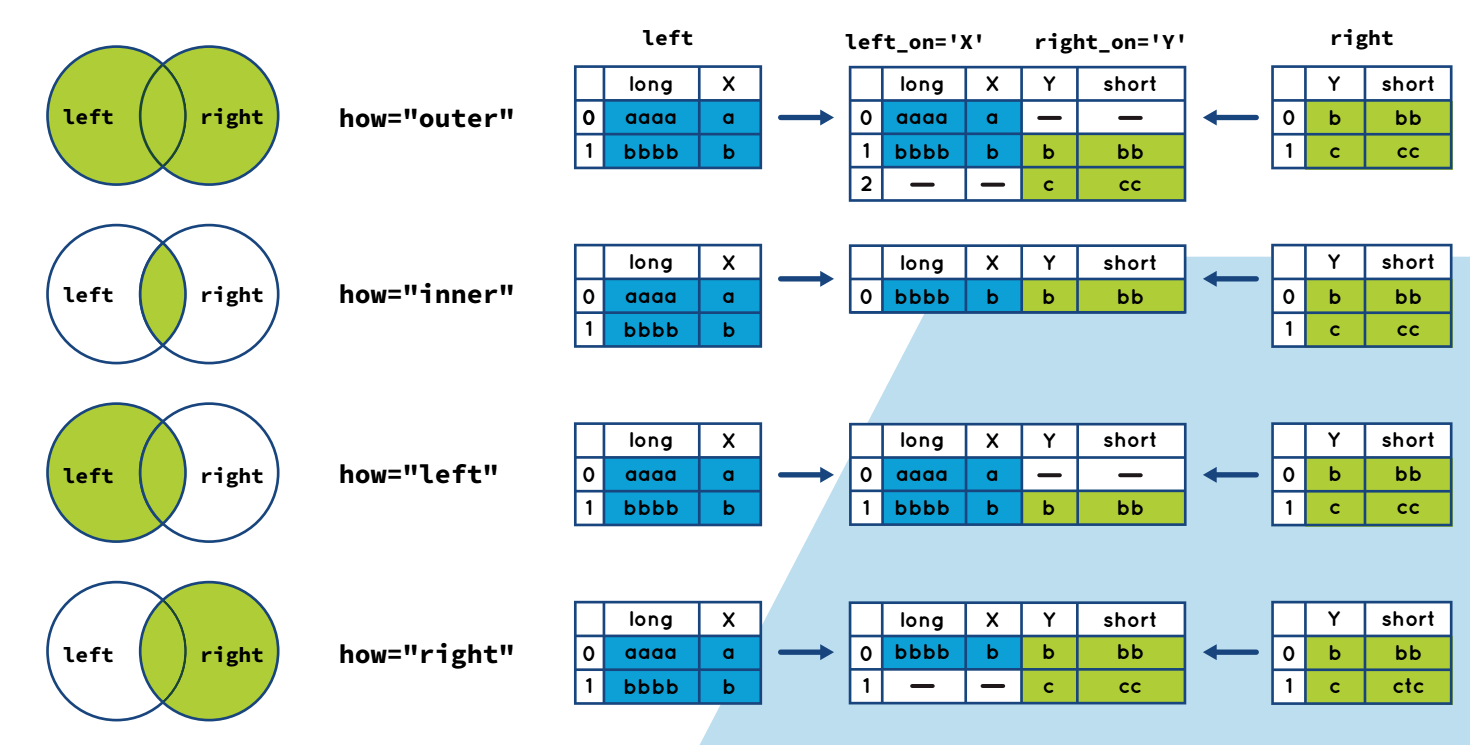
\includegraphics{Join.png}

    \begin{longtable}[]{@{}ccc@{}}
\toprule
\begin{minipage}[b]{0.29\columnwidth}\centering
SQL Sample\strut
\end{minipage} & \begin{minipage}[b]{0.34\columnwidth}\centering
Pandas Sample\strut
\end{minipage} & \begin{minipage}[b]{0.29\columnwidth}\centering
\strut
\end{minipage}\tabularnewline
\midrule
\endhead
\begin{minipage}[t]{0.29\columnwidth}\centering
\texttt{SELECT\ *}\texttt{FROM\ df1}\texttt{INNER\ JOIN\ df2}\texttt{ON\ df1.key\ =\ df2.key}\strut
\end{minipage} & \begin{minipage}[t]{0.34\columnwidth}\centering
\texttt{pd.merge(df1,\ df2,\ on=\textquotesingle{}key\textquotesingle{})}\strut
\end{minipage} & \begin{minipage}[t]{0.29\columnwidth}\centering
\strut
\end{minipage}\tabularnewline
\begin{minipage}[t]{0.29\columnwidth}\centering
\texttt{SELECT\ *}\texttt{FROM\ df1}\texttt{INNER\ JOIN\ df2}\texttt{ON\ df1.c7\ =\ df2.c5}\strut
\end{minipage} & \begin{minipage}[t]{0.34\columnwidth}\centering
\texttt{pd.merge(df1,\ df2,\ left\_on=\textquotesingle{}c7\textquotesingle{},right\_on=\textquotesingle{}c5\textquotesingle{})}\strut
\end{minipage} & \begin{minipage}[t]{0.29\columnwidth}\centering
\strut
\end{minipage}\tabularnewline
\bottomrule
\end{longtable}

    \hypertarget{time-functionality}{%
\subsection{6.Time functionality}\label{time-functionality}}

    In order to have possibility to use time related functionalities, we
need help \texttt{Pandas} understand which columns are to be treated as
time. Of course, the columns should be in for that converting them to
time format is possible. For details, please check and review
\href{http://pandas.pydata.org/pandas-docs/stable}{Pandas
documentation}. If you manage to let \texttt{Pandas} know properly which
column(s) to be time related column(s), they will end up having
\texttt{datetime64{[}ns{]}} format. \texttt{.dtypes} on dataframe
provides you with columns formats. Pass date related column(s) you need
to \texttt{parse\_dates} to \texttt{read\_csv} or \texttt{read\_excel}
functions. Check Pandas documentation for more details.

Doing so, you can apply \texttt{.dt} on column to have date - time
selection like \texttt{dt.dayofweek} \texttt{dt.minute} \texttt{dt.hour}
\texttt{dt.second} \texttt{dt.quarter} \texttt{dt.month}
\texttt{dt.month\_name} \texttt{dt.weekday\_name} \texttt{dt.weekday}
\texttt{dt.weekofyear} \texttt{dt.year}

\hypertarget{how-to-get-current-date-time-using-pandas}{%
\subsubsection{How to get current date time using
pandas?}\label{how-to-get-current-date-time-using-pandas}}

\texttt{pd.datetime.now()} \texttt{pd.datetime.now().date()}
\texttt{pd.datetime.now().year} \texttt{pd.datetime.now().month}
\texttt{pd.datetime.now().day} \texttt{pd.datetime.now().hour}
\texttt{pd.datetime.now().minute} \texttt{pd.datetime.now().second}
\texttt{pd.datetime.now().microsecond}

Again, check Pandas documentation for more! Here, we assume
\texttt{sdate} column to have \texttt{datetime64{[}ns{]}} format.

    \begin{longtable}[]{@{}ccc@{}}
\toprule
\begin{minipage}[b]{0.29\columnwidth}\centering
\strut
\end{minipage} & \begin{minipage}[b]{0.34\columnwidth}\centering
SQL Sample\strut
\end{minipage} & \begin{minipage}[b]{0.29\columnwidth}\centering
Pandas Sample\strut
\end{minipage}\tabularnewline
\midrule
\endhead
\begin{minipage}[t]{0.29\columnwidth}\centering
sysdate - n\strut
\end{minipage} & \begin{minipage}[t]{0.34\columnwidth}\centering
\texttt{SELECT\ *}\texttt{FROM\ df}\texttt{WHERE\ sdate\textgreater{}\ sysdate-5}\strut
\end{minipage} & \begin{minipage}[t]{0.29\columnwidth}\centering
\texttt{df{[}df{[}\textquotesingle{}sdate\textquotesingle{}{]}.dt.date()\textgreater{}\ \ pd.datetime.now().date()-5{]}}\strut
\end{minipage}\tabularnewline
\begin{minipage}[t]{0.29\columnwidth}\centering
month\strut
\end{minipage} & \begin{minipage}[t]{0.34\columnwidth}\centering
\texttt{SELECT\ *}\texttt{FROM\ df}\texttt{WHERE\ sdate\ in\ Q1}\strut
\end{minipage} & \begin{minipage}[t]{0.29\columnwidth}\centering
\texttt{df{[}(df.sdate.dt.month\ \textgreater{}=\ 1)\ \&\ (df.sdate.dt.month\ \textless{}=\ 3){]}}\strut
\end{minipage}\tabularnewline
\begin{minipage}[t]{0.29\columnwidth}\centering
between\strut
\end{minipage} & \begin{minipage}[t]{0.34\columnwidth}\centering
\texttt{SELECT\ *}\texttt{FROM\ t}\texttt{WHERE\ to\_char(sdate,\textquotesingle{}yyyy\textquotesingle{})\ between\ 1998\ AND\ 2018}\strut
\end{minipage} & \begin{minipage}[t]{0.29\columnwidth}\centering
\texttt{t{[}(t.sdate.dt.year\ \textgreater{}=\ 1998)\ \&\ (t.sdate.dt.year\ \textless{}=\ 2018){]}}\strut
\end{minipage}\tabularnewline
\begin{minipage}[t]{0.29\columnwidth}\centering
\strut
\end{minipage} & \begin{minipage}[t]{0.34\columnwidth}\centering
\texttt{SELECT\ *}\texttt{FROM\ t}\texttt{WHERE\ to\_char(sdate\ ,\textquotesingle{}day\textquotesingle{})=\ \textquotesingle{}Friday\textquotesingle{}}\strut
\end{minipage} & \begin{minipage}[t]{0.29\columnwidth}\centering
\texttt{df{[}df.sdate.dt.day\_name()\ ==\ \textquotesingle{}Friday\textquotesingle{}{]}}\strut
\end{minipage}\tabularnewline
\bottomrule
\end{longtable}

    \hypertarget{string-related-functionality-like-like-substr}{%
\subsection{\texorpdfstring{7. String related functionality like
\texttt{like},
\texttt{Substr}}{7. String related functionality like like, Substr}}\label{string-related-functionality-like-like-substr}}

    For columns with \texttt{string} content, we could access string related
funftionality by applying \texttt{.str} on column. Here are few samples:
\texttt{str.contains} -
\href{https://pandas.pydata.org/pandas-docs/stable/reference/api/pandas.Series.str.contains.html?}{contains}
options :
\texttt{Series.str.contains(pat,\ case=True,\ flags=0,\ na=nan,\ regex=True)}
\texttt{str.upper} \texttt{str.lower} \texttt{str.extract}
\texttt{str.extractall} \texttt{str.find} \texttt{str.findall}
\texttt{str.len} \texttt{str.replace} \texttt{str.slice}
\texttt{str.split} \texttt{str.strip}

Check
\href{https://pandas.pydata.org/pandas-docs/stable/search.html?q=.str.\&check_keywords=yes\&area=default}{Pandas
documentation} for more!

    \begin{longtable}[]{@{}ccc@{}}
\toprule
\begin{minipage}[b]{0.29\columnwidth}\centering
\strut
\end{minipage} & \begin{minipage}[b]{0.34\columnwidth}\centering
SQL Sample\strut
\end{minipage} & \begin{minipage}[b]{0.29\columnwidth}\centering
Pandas Sample\strut
\end{minipage}\tabularnewline
\midrule
\endhead
\begin{minipage}[t]{0.29\columnwidth}\centering
substr\strut
\end{minipage} & \begin{minipage}[t]{0.34\columnwidth}\centering
\texttt{SELECT\ *}\texttt{FROM\ tips}\texttt{WHERE\ substr(time,1,2)\ \ =\ \textquotesingle{}Di\textquotesingle{}}\strut
\end{minipage} & \begin{minipage}[t]{0.29\columnwidth}\centering
\texttt{tips{[}tips{[}\textquotesingle{}time\textquotesingle{}{]}.str{[}:2{]}\ ==\ \textquotesingle{}Di\textquotesingle{}{]}}\strut
\end{minipage}\tabularnewline
\begin{minipage}[t]{0.29\columnwidth}\centering
like\strut
\end{minipage} & \begin{minipage}[t]{0.34\columnwidth}\centering
\texttt{SELECT\ *}\texttt{FROM\ df}\texttt{WHERE\ Country\ \ like\ \textquotesingle{}\%IR\%\textquotesingle{}}\strut
\end{minipage} & \begin{minipage}[t]{0.29\columnwidth}\centering
\texttt{df{[}df{[}\textquotesingle{}Country\textquotesingle{}{]}.str.contains(\textquotesingle{}IR\textquotesingle{})\ ==\ True{]}}\strut
\end{minipage}\tabularnewline
\begin{minipage}[t]{0.29\columnwidth}\centering
like\strut
\end{minipage} & \begin{minipage}[t]{0.34\columnwidth}\centering
\texttt{SELECT\ *}\texttt{FROM\ df}\texttt{WHERE\ Country\ \ like\ \textquotesingle{}IR\%\textquotesingle{}}\strut
\end{minipage} & \begin{minipage}[t]{0.29\columnwidth}\centering
\texttt{df{[}df{[}\textquotesingle{}Country\textquotesingle{}{]}.str.startswith(\textquotesingle{}IR\textquotesingle{})\ ==\ True{]}}\strut
\end{minipage}\tabularnewline
\begin{minipage}[t]{0.29\columnwidth}\centering
like\strut
\end{minipage} & \begin{minipage}[t]{0.34\columnwidth}\centering
\texttt{SELECT\ *}\texttt{FROM\ df}\texttt{WHERE\ Country\ \ like\ \textquotesingle{}\%AN\textquotesingle{}}\strut
\end{minipage} & \begin{minipage}[t]{0.29\columnwidth}\centering
\texttt{df{[}df{[}\textquotesingle{}Country\textquotesingle{}{]}.str.endswith(\textquotesingle{}AN\textquotesingle{})\ ==\ True{]}}\strut
\end{minipage}\tabularnewline
\begin{minipage}[t]{0.29\columnwidth}\centering
in\strut
\end{minipage} & \begin{minipage}[t]{0.34\columnwidth}\centering
\texttt{SELECT\ *}\texttt{FROM\ df}\texttt{WHERE\ City\ in\ (\textquotesingle{}TEHRAN\textquotesingle{},\ \textquotesingle{}BERLIN\textquotesingle{},\textquotesingle{}STOKHOLM\textquotesingle{})}\strut
\end{minipage} & \begin{minipage}[t]{0.29\columnwidth}\centering
\texttt{df{[}df{[}\textquotesingle{}City\textquotesingle{}{]}.isin({[}\textquotesingle{}TEHRAN\textquotesingle{},\ \textquotesingle{}BERLIN\textquotesingle{},\textquotesingle{}STOKHOLM\textquotesingle{}{]})}\strut
\end{minipage}\tabularnewline
\begin{minipage}[t]{0.29\columnwidth}\centering
regex\strut
\end{minipage} & \begin{minipage}[t]{0.34\columnwidth}\centering
\texttt{SELECT\ last\_name}\texttt{FROM\ contacts}\texttt{WHERE\ REGEXP\_LIKE\ (last\_name,\ \textquotesingle{}\^{}A(*)\textquotesingle{})}\strut
\end{minipage} & \begin{minipage}[t]{0.29\columnwidth}\centering
\texttt{contacts{[}contacts{[}\textquotesingle{}last\_name\textquotesingle{}{]}.str.contains(\textquotesingle{}\^{}A(*)\textquotesingle{}){]}}\strut
\end{minipage}\tabularnewline
\begin{minipage}[t]{0.29\columnwidth}\centering
regex\strut
\end{minipage} & \begin{minipage}[t]{0.34\columnwidth}\centering
\texttt{SELECT\ c1}\texttt{FROM\ t}\texttt{WHERE\ REGEXP\_LIKE(c1,\textquotesingle{}({[}A-Z{]}{[}\textbackslash{}d{]}\{4\})\textquotesingle{})}\strut
\end{minipage} & \begin{minipage}[t]{0.29\columnwidth}\centering
\texttt{t{[}t{[}\textquotesingle{}c1\textquotesingle{}{]}.str.contains(({[}A-Z{]}{[}\textbackslash{}d{]}\{4\})){]}}\strut
\end{minipage}\tabularnewline
\begin{minipage}[t]{0.29\columnwidth}\centering
regex\strut
\end{minipage} & \begin{minipage}[t]{0.34\columnwidth}\centering
\texttt{SELECT\ upper(trim(to\_char(LAC,\textquotesingle{}xxxxx\textquotesingle{}))\ \textbackslash{}\textbackslash{}\textquotesingle{}-\textquotesingle{}\ \textbackslash{}\textbackslash{}\ trim(to\_char(CI,\textquotesingle{}xxxxx\textquotesingle{})))\ AS\ "LAC-CI(HEX)"}\texttt{FROM\ t}\strut
\end{minipage} & \begin{minipage}[t]{0.29\columnwidth}\centering
\texttt{t\ =\ t{[}\textquotesingle{}LAC\textquotesingle{},\textquotesingle{}CI\textquotesingle{}{]}.apply(lambda\ x:\ x.astype(str).map(lambda\ x:\ int(x,\ base=16)))}\texttt{t.assig(LAC-CI(HEX)\ =\ t{[}\textquotesingle{}LAC\textquotesingle{}{]}+\textquotesingle{}-\textquotesingle{}+t{[}\textquotesingle{}CI\textquotesingle{}{]}}\strut
\end{minipage}\tabularnewline
\bottomrule
\end{longtable}

PS: Consider to replace \texttt{\textbackslash{}\textbackslash{}} with
\texttt{\textbar{}\textbar{}} in your query.
\texttt{\textbar{}\textbar{}} provide concatenation functonality in SQL,
but symbol could not be rendered and I put
\texttt{\textbackslash{}\textbackslash{}} for now!

    \hypertarget{oracles-row_number-analytic-function}{%
\subparagraph{Oracle's ROW\_NUMBER() analytic
function}\label{oracles-row_number-analytic-function}}

    \begin{longtable}[]{@{}ccc@{}}
\toprule
\begin{minipage}[b]{0.29\columnwidth}\centering
SQL Sample\strut
\end{minipage} & \begin{minipage}[b]{0.34\columnwidth}\centering
Pandas Sample\strut
\end{minipage} & \begin{minipage}[b]{0.29\columnwidth}\centering
\strut
\end{minipage}\tabularnewline
\midrule
\endhead
\begin{minipage}[t]{0.29\columnwidth}\centering
\texttt{SELECT\ *\ FROM\ (}\texttt{SELECT\ t.*,}\texttt{ROW\_NUMBER()\ OVER(PARTITION\ BY\ day\ ORDER\ BY\ total\_bill\ DESC)\ AS\ r}\texttt{FROM\ tips\ t}\texttt{)}\texttt{WHERE\ r\ \textless{}\ 3}\texttt{ORDER\ BY\ day,\ r;}\strut
\end{minipage} & \begin{minipage}[t]{0.34\columnwidth}\centering
\texttt{(tips.assign(r=tips.sort\_values({[}\textquotesingle{}total\_bill\textquotesingle{}{]},ascending=False)}\texttt{.groupby({[}\textquotesingle{}day\textquotesingle{}{]})}\texttt{.cumcount()+1)}\texttt{.query(\textquotesingle{}r\ \textless{}\ 3\textquotesingle{})}\texttt{.sort\_values({[}\textquotesingle{}day\textquotesingle{},\ \textquotesingle{}r\textquotesingle{}{]}))}\strut
\end{minipage} & \begin{minipage}[t]{0.29\columnwidth}\centering
\strut
\end{minipage}\tabularnewline
\bottomrule
\end{longtable}

    \hypertarget{to-check-for-missing-values}{%
\subsection{\texorpdfstring{To check for missing values
}{To check for missing values  }}\label{to-check-for-missing-values}}

\begin{itemize}
\tightlist
\item
  \texttt{df.notnull()} Use to Drop Missing Values
\item
  \texttt{df.dropna()} Filling Missing Values --- Direct Replace
\item
  \texttt{df.fillna()}
\end{itemize}

    Besides
\href{https://pandas.pydata.org/pandas-docs/stable/getting_started/comparison/comparison_with_sql.html}{Pandas
comparison with SQL}, I also get ideas from following references: 1.
\url{https://hackernoon.com/pandas-cheatsheet-for-sql-people-part-1-2976894acd0}
2.
\url{https://medium.com/jbennetcodes/how-to-rewrite-your-sql-queries-in-pandas-and-more-149d341fc53e}
3. \url{https://www.kaggle.com/anagharumade/thinking-like-sql-in-pandas}
4.
\url{https://medium.com/fintechexplained/did-you-know-pandas-can-do-so-much-f65dc7db3051}
5.
\url{https://towardsdatascience.com/10-python-pandas-tricks-that-make-your-work-more-efficient-2e8e483808ba}


    % Add a bibliography block to the postdoc
    
    
    
\end{document}
